\documentclass[12pt,a4paper]{article}

% ==== Paquetes básicos ====
\usepackage[T1]{fontenc}
\usepackage[utf8]{inputenc}
\usepackage[spanish,es-tabla]{babel}
\usepackage{lmodern}
\usepackage{geometry}
\usepackage{setspace}
\usepackage{parskip}
\usepackage{hyperref}
\usepackage{graphicx}
\usepackage{booktabs}
\usepackage{float}
\usepackage{background}
\usepackage{tabularx}
\usepackage{array}
\usepackage[table]{xcolor}
\usepackage{csquotes}
\usepackage{amsmath}
\usepackage{subcaption}
\usepackage{threeparttable}
\usepackage[authoryear]{natbib}

\geometry{margin=2.5cm}
\onehalfspacing
\hypersetup{
  colorlinks=true,
  linkcolor=blue,
  citecolor=blue,
  urlcolor=blue
}

\begin{document}

\backgroundsetup{contents={}}

% ==== Portada ====
\begin{titlepage}
  \centering

  \begin{minipage}{0.45\textwidth}
    \raggedright
    
\includegraphics[width=0.8\textwidth]{Imagenes/fce_logo.png}
  \end{minipage}%
  \begin{minipage}{0.45\textwidth}
    \raggedleft
    
\includegraphics[width=0.4\textwidth]{Imagenes/unrc_logo.png}
  \end{minipage}

  \vspace{1.5cm}

  {\Large \textbf{Universidad Nacional de Río Cuarto} \\[2pt]}
  {\Large \textbf{Facultad de Ciencias Económicas} \\[2pt]}\par\vspace{2.5cm}

  {\Large \textit{Usos empresariales de inteligencia artificial y productividad laboral: evidencia país--sector para la Unión Europea}}\\[3.5cm]

  \begin{tabular}{@{}ll}
    Alumno: & Facundo Díaz Larrarte \\
    DNI: & 43.475.555 \\
    Registro Universitario: & \textit{[completar]} \\
    Email: & fdiazlarrarte@mail.com \\
    Director: & Ernesto Bosch \\
    Codirectora: & Ana Vianco \\
    Fecha de presentación: & \textit{[completar]} \\
  \end{tabular}

  \vspace{2cm}
  {\Large \textbf{Trabajo Final de Grado}}\\[0.3cm]
  {\Large \textbf{Licenciatura en Economía}}

  \vfill
  {\large Ciudad de Río Cuarto, Argentina}

\end{titlepage}

\newpage
\tableofcontents

\newpage
\listoftables

\newpage
\listoffigures

\newpage
\section*{Resumen}
\addcontentsline{toc}{section}{Resumen}

El presente Trabajo Final de Grado analiza la relación entre los usos empresariales de inteligencia artificial y la productividad laboral aparente en sectores económicos de la Unión Europea. A partir de información secundaria de Eurostat, se construye una base país--sector--año que combina indicadores de adopción y usos de inteligencia artificial con datos de valor agregado y personas ocupadas provenientes de estadísticas estructurales empresariales. El objetivo es estudiar la heterogeneidad sectorial de la adopción tecnológica y estimar su asociación con la productividad, distinguiendo entre correlaciones en niveles y variaciones dentro de cada unidad país--sector.

El enfoque es cuantitativo, longitudinal, observacional y no experimental. La estrategia empírica propuesta utiliza modelos de datos de panel con efectos fijos, manteniendo una interpretación asociativa y evitando inferencias causales no respaldadas por el diseño. Los resultados preliminares muestran una asociación positiva entre adopción de inteligencia artificial y productividad en niveles, pero esa relación se debilita al controlar por diferencias permanentes entre unidades país--sector y shocks país--año. Esta diferencia sugiere la necesidad de distinguir entre adopción tecnológica y realización productiva, así como de considerar la heterogeneidad sectorial, los activos complementarios y las limitaciones de medición.

\vspace{1.5cm}
\noindent\textbf{Palabras clave:} inteligencia artificial; productividad laboral; adopción tecnológica; datos de panel; Unión Europea.

\newpage

\section{Introducción}

\subsection{Planteo del problema}

La difusión reciente de tecnologías de inteligencia artificial (IA) ha reactivado el debate sobre su capacidad para modificar procesos productivos, reducir costos, mejorar la calidad de las decisiones empresariales y elevar la productividad. Sin embargo, la adopción de una tecnología y la obtención de resultados económicos observables son fenómenos diferentes. Una empresa puede declarar el uso de IA sin que ello implique necesariamente una transformación profunda de sus procesos, una mejora inmediata de eficiencia o un aumento medible de la productividad.

Desde la perspectiva económica, la incorporación de IA puede entenderse como una decisión de adopción tecnológica cuyo impacto depende de las tareas afectadas, la organización interna, las capacidades del personal, la infraestructura digital, la calidad de los datos, los costos de implementación y el horizonte temporal de maduración. La literatura sobre tecnologías de propósito general y curva J de productividad sostiene que los beneficios de ciertas innovaciones pueden observarse con demora, luego de inversiones complementarias y reorganización empresarial \citep{brynjolfsson2021productivity}.

La pregunta principal de este trabajo es: \textit{¿cómo varían la adopción y los usos empresariales de inteligencia artificial entre los sectores económicos de la Unión Europea, y en qué medida esas diferencias se asocian con distintos niveles y variaciones de productividad laboral?}

Esta pregunta no busca demostrar que la IA cause por sí sola aumentos de productividad. El propósito es más acotado: reconstruir evidencia empírica comparable, estudiar patrones de adopción y usos funcionales, y evaluar si la asociación positiva que puede observarse entre unidades estructuralmente distintas se mantiene al analizar variaciones dentro de cada país--sector.

\subsection{Delimitación del tema y del área de estudio}

El trabajo se inscribe en la microeconomía aplicada, la economía de la empresa y la economía del cambio tecnológico. El análisis utiliza información secundaria de Eurostat para los 27 países de la Unión Europea, nueve sectores de actividad definidos según NACE Rev. 2 y los años 2021, 2023 y 2024.

La unidad de observación es la combinación país--sector--año. La adopción de IA se mide mediante el porcentaje de empresas de diez o más personas ocupadas que declara utilizar al menos una tecnología de IA. Además, se consideran indicadores de intensidad y usos funcionales, tales como IA en organización de procesos o toma de decisiones, producción, logística, marketing y ventas, y seguridad informática.

La productividad laboral aparente se calcula como el cociente entre valor agregado y personas ocupadas:

\begin{equation}
  Productividad_{cst} =
  \frac{Valor\ agregado_{cst}}{Personas\ ocupadas_{cst}},
\end{equation}

donde $c$ identifica al país, $s$ al sector y $t$ al año. Este indicador no mide productividad total de los factores ni permite aislar por sí solo la contribución causal de la IA.

\subsection{Objetivo general}

Analizar cómo varían la adopción y los usos empresariales de inteligencia artificial entre sectores de la Unión Europea y estimar su asociación con la productividad laboral aparente, utilizando la adopción general como referencia y considerando la heterogeneidad productiva sectorial.

\subsection{Objetivos específicos}

\begin{itemize}
  \item Integrar en una base país--sector--año indicadores de IA, valor agregado y personas ocupadas de Eurostat.
  \item Describir la evolución y heterogeneidad de la adopción de IA por país, sector y año.
  \item Calcular y comparar la productividad laboral aparente entre las unidades analizadas.
  \item Estimar una asociación de referencia entre adopción general de IA y productividad mediante modelos de datos de panel.
  \item Comparar la adopción general con usos empresariales específicos de IA.
  \item Examinar si la relación entre IA y productividad presenta heterogeneidad sectorial.
  \item Evaluar la sensibilidad de los resultados frente a especificaciones alternativas, ponderaciones, valores extremos y tratamiento de precios.
  \item Explicitar las limitaciones de medición e interpretación del diseño empírico.
\end{itemize}

\subsection{Hipótesis de trabajo}

La hipótesis de referencia sostiene que una mayor adopción empresarial de IA se asocia con una mayor productividad laboral aparente. La primera hipótesis central plantea que dicha asociación no es uniforme entre funciones empresariales: los usos vinculados con procesos internos, decisiones, producción y logística podrían relacionarse más estrechamente con productividad que la adopción general o que usos de apoyo y comercialización. La segunda hipótesis central sostiene que la asociación entre IA y productividad es heterogénea entre sectores debido a diferencias en tareas, tecnologías productivas y capacidades complementarias.

Estas hipótesis son asociativas. No se formulan como afirmaciones causales ni como resultados garantizados.

\subsection{Importancia del estudio}

El aporte del trabajo reside en construir una base reproducible con fuentes oficiales, distinguir entre adopción general y usos específicos de IA, comparar correlaciones en niveles con variaciones dentro de cada unidad país--sector y discutir la heterogeneidad sectorial de la relación IA--productividad. En una tesina de grado, la contribución esperada no consiste en resolver de manera definitiva la identificación causal, sino en presentar un análisis empírico transparente, metodológicamente defendible y prudente en su interpretación.

\subsection{Limitaciones del estudio}

El diseño permite estudiar asociaciones, pero no identifica de manera concluyente el efecto causal de la IA. Entre las principales limitaciones se encuentran el reducido número de años comparables, el nivel agregado país--sector, la posible causalidad inversa, la omisión de capacidades organizacionales no observadas y la medición de productividad mediante valor agregado monetario corriente.

Los datos no permiten determinar si una empresa concreta eligió la herramienta adecuada, si implementó bien la IA, cuánto gastó, cuánto ahorró o cuál fue su retorno económico. Por lo tanto, una combinación de elevada adopción y débil crecimiento de productividad puede sugerir una brecha de realización productiva compatible con distintos mecanismos, pero no demuestra por sí sola un uso incorrecto de la tecnología.

\section{Marco teórico y antecedentes}

\subsection{Adopción tecnológica, enfoque de tareas y complementariedades}

La incorporación de inteligencia artificial en el ámbito empresarial se inscribe dentro de los procesos de adopción y difusión tecnológica analizados tradicionalmente por la teoría económica. Desde la perspectiva de la empresa, la decisión de adoptar una nueva tecnología responde a un cálculo de optimización intertemporal bajo incertidumbre, en el cual se comparan los costos esperados de adquisición, instalación, aprendizaje y reorganización con los flujos de beneficios derivados de mejoras en eficiencia, reducción de costos operativos, mayor velocidad de procesamiento de información o generación de nuevos productos y servicios.

Sin embargo, las tecnologías digitales complejas no operan en el vacío ni sustituyen automáticamente sectores o actividades en su totalidad. En consonancia con la literatura contemporánea de economía laboral y del cambio tecnológico, la producción puede descomponerse analíticamente en una secuencia de tareas cognitivas y manuales, rutinarias y no rutinarias. Las herramientas de IA interactúan directamente con tareas específicas: algunas son susceptibles de automatización directa (cuando los algoritmos reemplazan la intervención humana en procesos estandarizados), mientras que en otras la tecnología actúa como un factor de asistencia o aumento de las capacidades de los trabajadores, incrementando la calidad de las decisiones o la velocidad de ejecución.

Esta especificidad de las tareas fundamenta la necesidad de examinar la heterogeneidad funcional de la adopción de IA. No es esperable que cualquier uso empresarial de IA genere el mismo tipo de impacto sobre el valor agregado por trabajador. En particular, conviene distinguir analíticamente entre:
\begin{enumerate}
    \item \textbf{Usos de gestión y toma de decisiones:} herramientas aplicadas a la organización de procesos internos, planificación operativa, análisis predictivo de demanda y soporte analítico a la dirección estratégica.
    \item \textbf{Usos en producción directa y logística:} algoritmos orientados al control de calidad en tiempo real, mantenimiento predictivo de maquinaria, optimización de flujos de cadena de suministro y gestión automatizada de inventarios.
    \item \textbf{Usos periféricos o de comercialización:} aplicaciones orientadas a marketing, perfilado y segmentación de clientes, publicidad dirigida o soporte inicial de seguridad informática.
\end{enumerate}

Desde el punto de vista de la teoría de la producción, los usos integrados en el núcleo operativo de las empresas (procesos, decisiones, producción física y logística) presentan un vínculo teórico más directo con la reducción sustantiva de tiempos muertos, desperdicios y costos de coordinación, lo que debería traducirse con mayor probabilidad en incrementos mensurables de productividad laboral. Por el contrario, los usos periféricos o auxiliares pueden responder a exigencias competitivas de diferenciación comercial o cumplimiento de estándares básicos de TIC sin transformar necesariamente la eficiencia estructural de los procesos centrales.

\subsection{Tecnologías de propósito general y la curva J de productividad}

Diversos autores conceptualizan a la inteligencia artificial como una tecnología de propósito general (\textit{General Purpose Technology} o GPT), caracterizada por su omnipresencia potencial en múltiples sectores de la economía, su dinamismo innovativo intrínseco y su capacidad para desencadenar innovaciones complementarias en las organizaciones usuarias.

Una característica fundamental de las tecnologías de propósito general es la desconexión temporal entre su difusión inicial y su impacto agregado en las estadísticas económicas. En su formulación teórica sobre la paradoja de la productividad de las nuevas tecnologías, \citet{brynjolfsson2021productivity} desarrollan el marco de la \textbf{curva J de productividad}. Este modelo postula que la adopción efectiva de una GPT requiere acumular cuantiosas inversiones en activos complementarios intangibles, entre los que se destacan:
\begin{itemize}
    \item el rediseño profundo de los flujos de trabajo organizacionales;
    \item el desarrollo de nuevas habilidades y capacitación del capital humano;
    \item la acumulación, saneamiento e interoperabilidad de grandes volúmenes de datos;
    \item el cambio cultural y la adaptación de las prácticas de gestión empresarial.
\end{itemize}

Durante las fases iniciales de difusión de una tecnología como la IA, una proporción considerable del tiempo de trabajo y de los recursos de las empresas se desvía hacia la creación y ajuste de este capital intangible. Dado que las convenciones de contabilidad nacional registran con frecuencia estos esfuerzos como gastos corrientes de operación y no como acumulación formal de activos, la productividad aparente medida puede estancarse o incluso caer transitoriamente, dibujando la parte descendente de la ``J''. Solo cuando el stock de intangibles complementarios alcanza un umbral crítico de maduración y se articula eficazmente con los procesos productivos, la empresa comienza a cosechar los retornos tangibles, permitiendo que la productividad medida crezca con celeridad.

Este marco teórico reviste una importancia metodológica central para este trabajo: advierte que la ausencia de una asociación temporal positiva y contemporánea entre aumentos de adopción de IA y crecimiento de la productividad aparente en el corto plazo no constituye evidencia de ineficacia tecnológica, sino que resulta enteramente compatible con la presencia de costos de ajuste e inversiones complementarias no observadas en plena fase de gestación.

\subsection{Evidencia empírica sobre IA y productividad en Europa}

La literatura empírica sobre la relación entre IA y productividad ha proliferado en los últimos años, dividiéndose entre estudios a nivel de empresa (\textit{firm-level}) y análisis agregados a escala sectorial o macroeconómica.

En el plano microeconómico, \citet{czarnitzki2023firm} examinan una muestra representativa de empresas en Alemania y constatan que aquellas firmas que incorporan soluciones de IA exhiben niveles sistemáticamente más elevados de productividad laboral frente a empresas similares no adoptantes. Sin embargo, los autores enfatizan que esta prima de productividad no es automática: está fuertemente condicionada por la intensidad en tecnologías de información preexistentes y por la disponibilidad de trabajadores altamente calificados capaces de interactuar con dichas tecnologías. Por su parte, el trabajo de \citet{aldasoro2026adoption}, elaborado para el Banco de Pagos Internacionales (BIS) a partir de una amplia encuesta de empresas europeas, halla una heterogeneidad sustancial en las respuestas productivas de las firmas. Concluyen que los efectos positivos en valor agregado se concentran en aquellas organizaciones que acompañan la adopción tecnológica con transformaciones profundas en sus prácticas de gobernanza y gestión corporativa.

A nivel agregado y sectorial, los estudios empíricos para la Unión Europea son más recientes y se sustentan en los datos armonizados de Eurostat. \citet{kadarova2026slovakia} analizan la adopción de IA en comparación entre Eslovaquia y el promedio de la UE-27, destacando la marcada disparidad estructural entre países miembros y la correlación positiva existente entre indicadores agregados de digitalización y niveles de productividad laboral. Asimismo, \citet{yilmaz2026dataset} construye una base país--sector para el período 2021--2025 y formula el concepto de la brecha de atribución de la IA (\textit{AI attribution wedge}), evidenciando que la rápida aceleración en las tasas de adopción reportadas por las empresas no encuentra un correlato inmediato en la dinámica de crecimiento de la productividad sectorial.

La coexistencia de resultados positivos en estudios microeconómicos y resultados moderados o nulos en agregaciones sectoriales obedece a un fenómeno clásico de selección y agregación: las encuestas microeconómicas capturan el desempeño de firmas pioneras o más productivas en la frontera (\textit{frontier firms}), mientras que los datos sectoriales consolidan el desempeño conjunto de líderes y rezagadas, amortiguando cualquier impacto agregado si la tecnología aún no alcanza una difusión profunda en la mediana de las unidades productivas.

\subsection{Desafíos econométricos e interpretación en datos de panel}

El estudio de la relación entre adopción tecnológica y productividad enfrenta serios desafíos de identificación que condicionan la estrategia empírica:
\begin{enumerate}
    \item \textbf{Causalidad inversa y endogeneidad por selección:} las empresas y sectores que presentan mayores niveles de productividad, mayor rentabilidad y mayores recursos de capital poseen simultáneamente mayores facilidades para afrontar los costos fijos y el riesgo que implica experimentar con tecnologías emergentes de IA. Por ende, una asociación positiva observada en un corte transversal no demuestra que la IA cause productividad, sino que puede reflejar que las unidades más productivas eligen adoptar más tecnología.
    \item \textbf{Heterogeneidad estructural no observada:} las diferencias institucionales, los regímenes regulatorios, las dotaciones iniciales de capital físico e intangibles y la composición del capital humano varían fuertemente entre países y sectores de actividad en la Unión Europea.
    \item \textbf{Shocks nominales y macroeconómicos:} el período reciente (2021--2024) estuvo signado por perturbaciones exógenas severas en Europa, incluyendo disrupciones en cadenas de suministro globales, presiones inflacionarias y la crisis energética derivada de la guerra en Ucrania, fenómenos que afectaron de modo heterogéneo a los deflactores y al valor agregado nominal entre sectores y países.
\end{enumerate}

Para mitigar estos problemas, la literatura econométrica estándar de datos de panel \citep{wooldridge2010econometric} recomienda recurrir al estimador dentro de entidad (\textit{within estimator}). La inclusión de efectos fijos de entidad país--sector ($\alpha_{cs}$) permite eliminar por completo cualquier factor no observable invariable en el tiempo que diferencie estructuralmente a una combinación país--sector de otra. Complementariamente, la incorporación de efectos fijos país--año ($\gamma_{ct}$) absorbe todos los shocks macroeconómicos y variaciones de precios comunes a todos los sectores de un determinado país en un año específico. De esta manera, el parámetro de interés identifica estrictamente si los cambios temporales en la tasa de adopción de IA al interior de un sector se corresponden con aceleraciones simultáneas en el ritmo de crecimiento de su productividad laboral.

\subsection{Aporte específico de este trabajo}

En el marco de la literatura expuesta, la presente tesina de grado se define como una \textbf{replicación y extensión metodológica} acotada y transparente. El trabajo no pretende implementar una estrategia de identificación cuasi-experimental exhaustiva que resuelva definitivamente la endogeneidad, sino aportar rigor analítico y claridad empírica a través de cuatro elementos distintivos:
\begin{itemize}
    \item Reconstrucción abierta y plenamente reproducible de una base de panel país--sector--año para la UE-27 a partir de microdatos oficiales agregados de Eurostat (SBS y TIC).
    \item Desagregación funcional de los indicadores de IA, evaluando de forma independiente la adopción general frente a usos concretos en procesos internos, decisiones, producción, logística, comercialización y seguridad.
    \item Contraste metodológico sistemático entre la correlación transversal en niveles y la estimación de efectos temporales con controles estrictos por heterogeneidad fija y shocks anuales.
    \item Análisis explícito de la heterogeneidad sectorial mediante interacciones econométricas y pruebas de robustez predefinidas.
\end{itemize}

La discusión de los resultados se estructura alrededor del concepto de \textbf{brecha de realización productiva}: la constatación descriptiva de una disonancia entre la velocidad de adopción tecnológica y el ritmo de generación de valor agregado medido. Esta brecha se interpreta como un patrón compatible con costos de ajuste, maduración de intangibles y complementariedades pendientes, manteniendo una estricta cautela interpretativa y evitando extrapolar juicios normativos sobre la eficiencia de empresas individuales a partir de información agregada sectorial.

\section{Datos y metodología}

\subsection{Fuentes de información}

El trabajo utiliza datos secundarios de Eurostat. Las fuentes principales son la base \texttt{isoc\_eb\_ai}, referida al uso de inteligencia artificial en empresas \citep{eurostat_ai}; la base \texttt{isoc\_eb\_ain2}, con indicadores complementarios sobre usos y características de la adopción \citep{eurostat_ain2}; y las estadísticas estructurales empresariales de Eurostat, utilizadas para obtener valor agregado y personas ocupadas \citep{eurostat_sbs}.

La cobertura principal comprende 27 países de la Unión Europea, nueve sectores NACE Rev. 2 y tres años: 2021, 2023 y 2024. La base analítica preliminar contiene 729 combinaciones teóricas de país, sector y año. De ellas, 667 cuentan con información central completa. La muestra balanceada preliminar contiene 209 unidades país--sector observadas en los tres años, equivalentes a 627 observaciones.

\subsection{Sectores considerados}

\begin{table}[H]
\centering
\caption{Sectores incluidos en el análisis}
\label{tab:sectores}
\begin{tabular}{ll}
\toprule
\textbf{Código} & \textbf{Sector} \\
\midrule
C & Industria manufacturera \\
F & Construcción \\
G & Comercio mayorista y minorista \\
H & Transporte y almacenamiento \\
I & Alojamiento y servicios de comida \\
J & Información y comunicación \\
L & Actividades inmobiliarias \\
M & Actividades profesionales, científicas y técnicas \\
N & Actividades administrativas y servicios auxiliares \\
\bottomrule
\end{tabular}
\end{table}

\subsection{Variables}

La variable dependiente es el logaritmo de la productividad laboral aparente, expresada inicialmente en miles de euros por persona ocupada. La transformación logarítmica reduce la influencia de valores extremos y permite interpretar aproximadamente los coeficientes como variaciones porcentuales.

Las variables explicativas de IA se expresan como porcentaje de empresas. La adopción general se mide con \texttt{ai\_any\_pct}. Como indicadores adicionales se consideran medidas de intensidad (dos o más y tres o más tecnologías) y usos funcionales en procesos, producción, logística, marketing y ventas, y seguridad informática. Cada indicador se analiza inicialmente en modelos separados para evitar combinar variables superpuestas o altamente correlacionadas sin justificación previa.

\subsection{Estrategia descriptiva}

La primera etapa del análisis describe la evolución de la adopción de IA y de la productividad laboral aparente por año y sector. También compara correlaciones en niveles con correlaciones de cambios entre 2021 y 2024. Esta distinción es central porque una asociación transversal positiva puede estar impulsada por diferencias estructurales persistentes entre países y sectores, mientras que las variaciones internas capturan otra dimensión del fenómeno.

\subsection{Estrategia econométrica}

La especificación principal propuesta es:

\begin{equation}
 \ln(Productividad_{cst}) =
 \beta IA_{cst} + \alpha_{cs} + \gamma_{ct} + \varepsilon_{cst},
\end{equation}

donde $c$ representa el país, $s$ el sector y $t$ el año. El término $\alpha_{cs}$ corresponde a efectos fijos de la unidad país--sector, que absorben diferencias permanentes de cada combinación. El término $\gamma_{ct}$ representa efectos fijos país--año, que capturan shocks comunes a todos los sectores de un país en un año determinado. Los errores estándar se agrupan por entidad país--sector.

También se estiman especificaciones comparativas con efectos fijos de país, sector y año, y con efectos fijos de país--sector y año. La estimación e interpretación de modelos de panel se apoya en criterios habituales de econometría aplicada \citep{wooldridge2010econometric}.

\subsection{Heterogeneidad sectorial}

La heterogeneidad sectorial se analiza descriptivamente y, como extensión econométrica, mediante interacciones entre el indicador de IA y sectores:

\begin{equation}
 \ln(Productividad_{cst}) =
 \beta IA_{cst}
 + \sum_{s \neq s_0} \delta_s(IA_{cst}\times Sector_s)
 + \alpha_{cs} + \gamma_{ct} + \varepsilon_{cst}.
\end{equation}

El sector $s_0$ funciona como categoría de referencia. La pendiente estimada para cada sector se obtiene como $\beta + \delta_s$. Dado que sólo se dispone de tres olas comparables, estos resultados deben interpretarse como evidencia exploratoria de heterogeneidad asociativa.

\subsection{Robustez prevista}

Las pruebas de robustez previstas incluyen comparar muestra balanceada y no balanceada, ponderar por personas ocupadas, examinar sensibilidad a valores extremos, utilizar efectos fijos alternativos, evaluar el tratamiento de precios o deflactores, estimar indicadores de IA por separado y validar los modelos con bibliotecas econométricas estándar. Estas pruebas deben definirse antes de seleccionar resultados para evitar elegir especificaciones únicamente por significatividad estadística.

\section{Resultados preliminares}

\subsection{Evolución agregada}

La exploración inicial indica que la adopción general media de IA en la muestra balanceada aumenta de 9,2\% en 2021 a 17,2\% en 2024. En el mismo período, la productividad laboral aparente nominal media pasa de 61,8 a 72,8 miles de euros corrientes por persona ocupada. La Tabla~\ref{tab:evolucion} resume estos indicadores.

\begin{table}[H]
\centering
\caption{Evolución de productividad e indicadores seleccionados de IA}
\label{tab:evolucion}
\scriptsize
\resizebox{\textwidth}{!}{%
\begin{tabular}{rrrrrrrr}
\toprule
\textbf{Año} & \textbf{Obs.} & \textbf{Prod. media} & \textbf{Prod. mediana} & \textbf{IA general} & \textbf{Procesos} & \textbf{Producción} & \textbf{Marketing} \\
\midrule
2021 & 209 & 61,8 & 44,4 & 9,2 & 4,0 & 2,0 & 2,6 \\
2023 & 209 & 67,9 & 51,5 & 10,0 & 4,0 & 2,3 & 2,8 \\
2024 & 209 & 72,8 & 54,3 & 17,2 & 6,1 & 3,9 & 6,2 \\
\bottomrule
\end{tabular}%
}
\begin{flushleft}
\footnotesize Nota: productividad en miles de euros corrientes por persona ocupada. Indicadores de IA en porcentaje de empresas. Muestra balanceada.
\end{flushleft}
\end{table}

\begin{figure}[H]
    \centering
    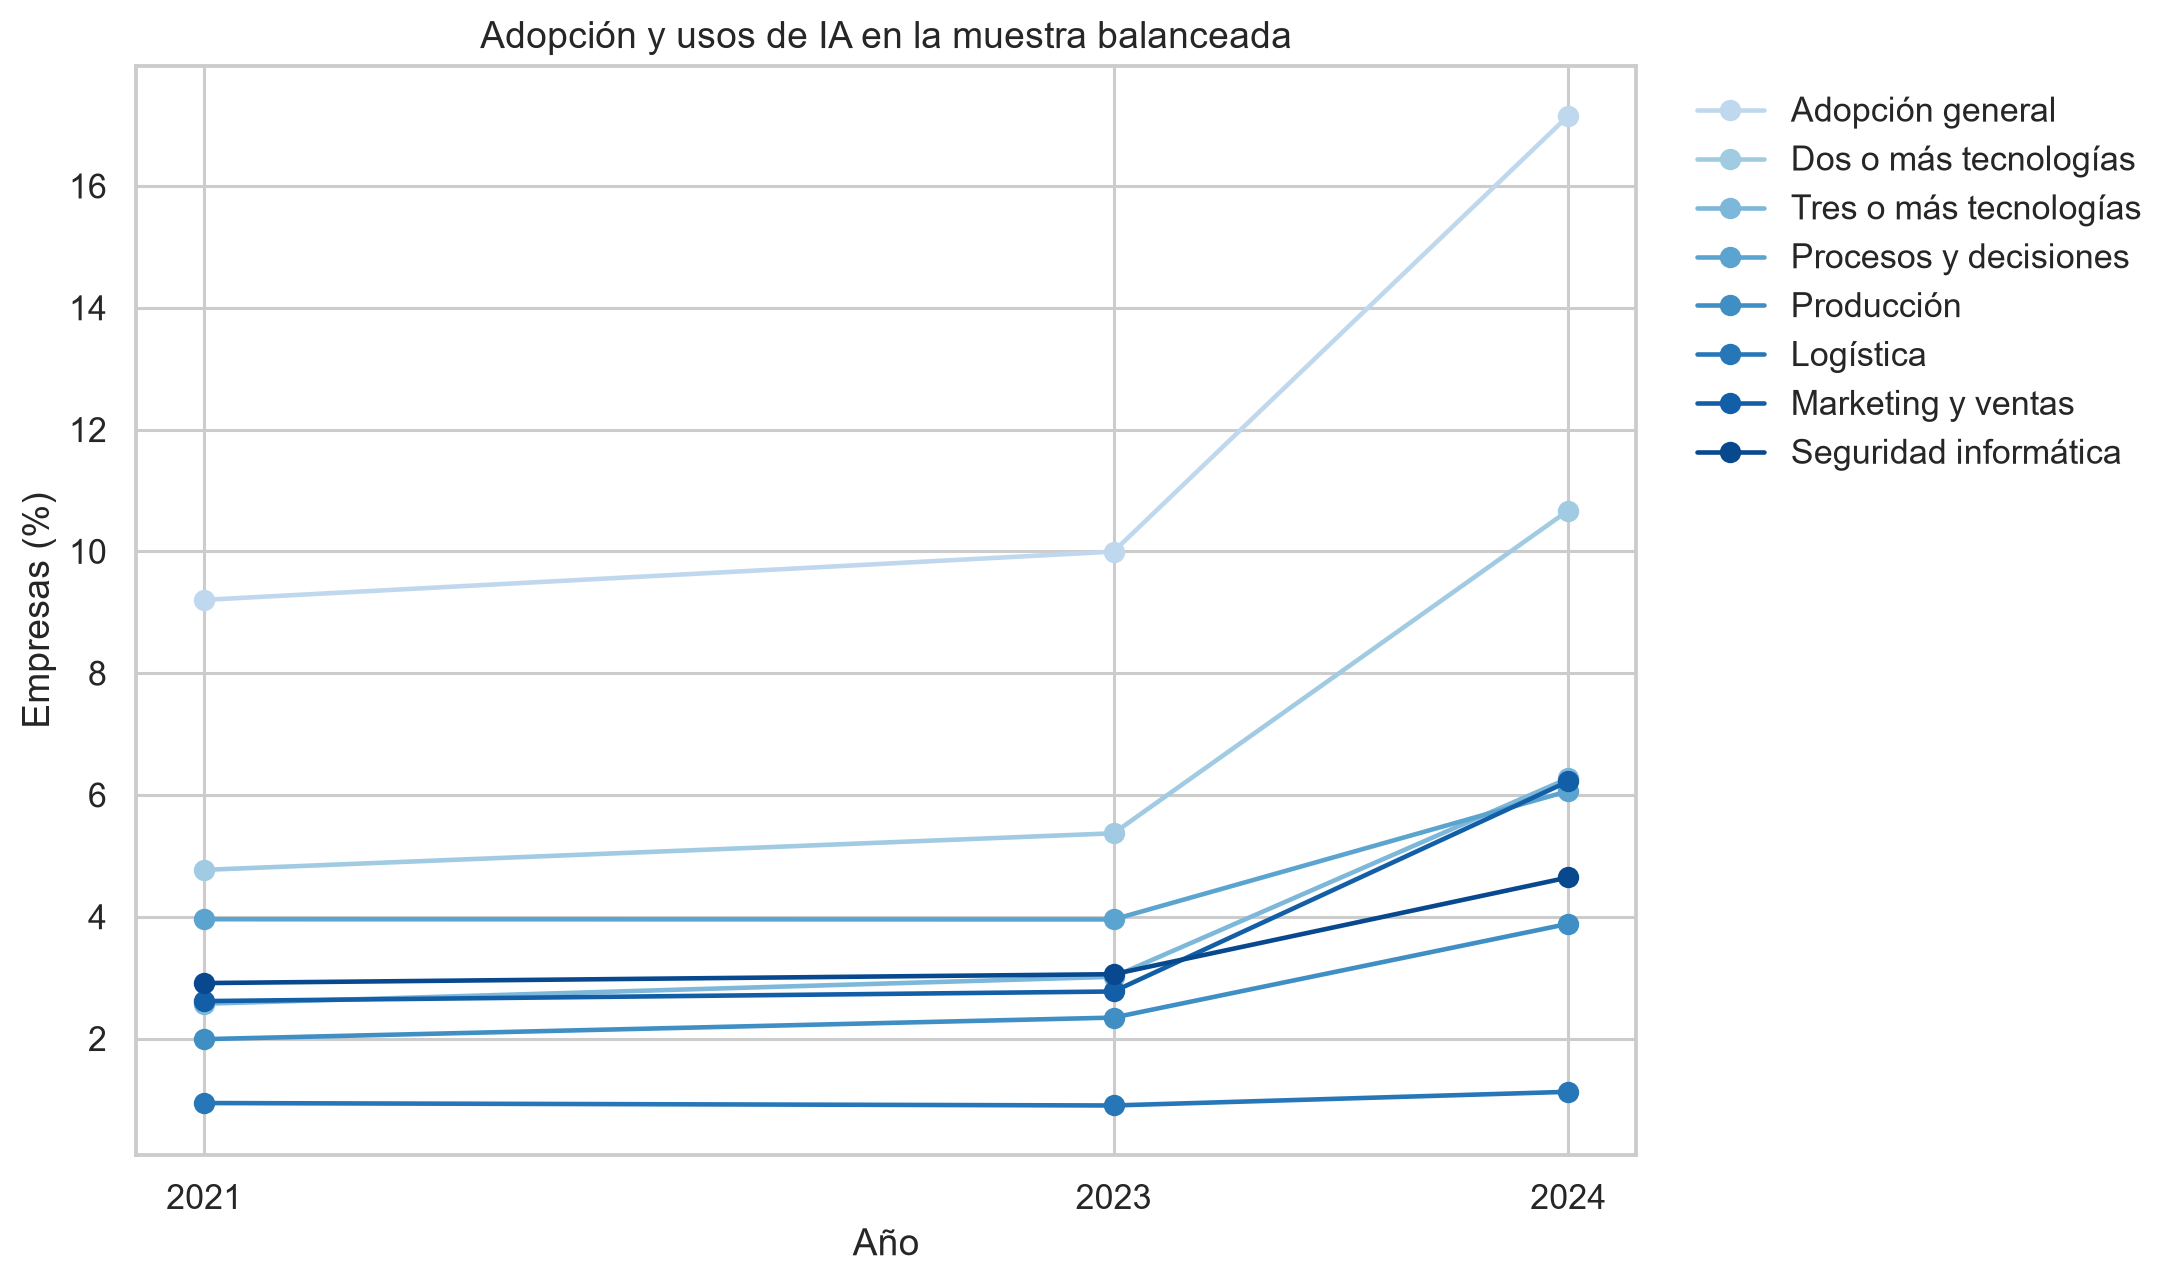
\includegraphics[width=0.95\linewidth]{../outputs/descriptivo_v0_1/figures/adopcion_ia_por_anio.png}
    \caption{Adopción y usos de IA por año}
    \label{fig:adopcion-anio}
\end{figure}

\subsection{Heterogeneidad sectorial descriptiva}

La adopción de IA presenta diferencias claras entre sectores. Información y comunicación muestra el mayor promedio de adopción general, seguido por actividades profesionales, científicas y técnicas. En el extremo opuesto se ubican alojamiento y servicios de comida, construcción y transporte. La Tabla~\ref{tab:sectores-resultados} y la Figura~\ref{fig:adopcion-sector} resumen esta heterogeneidad.

\begin{table}[H]
\centering
\caption{Adopción general de IA y productividad media por sector}
\label{tab:sectores-resultados}
\small
\begin{tabularx}{\textwidth}{lXrr}
\toprule
\textbf{Código} & \textbf{Sector} & \textbf{IA general} & \textbf{Prod. media} \\
\midrule
J & Información y comunicación & 33,0 & 118,6 \\
M & Actividades profesionales, científicas y técnicas & 18,7 & 67,9 \\
L & Actividades inmobiliarias & 11,9 & 119,4 \\
N & Actividades administrativas y servicios auxiliares & 10,5 & 35,8 \\
C & Industria manufacturera & 8,9 & 94,2 \\
G & Comercio mayorista y minorista & 8,5 & 53,0 \\
H & Transporte y almacenamiento & 7,6 & 60,6 \\
F & Construcción & 5,0 & 52,8 \\
I & Alojamiento y servicios de comida & 4,7 & 28,4 \\
\bottomrule
\end{tabularx}
\begin{flushleft}
\footnotesize Nota: IA general en porcentaje de empresas; productividad en miles de euros corrientes por persona ocupada. Promedios de la muestra balanceada.
\end{flushleft}
\end{table}

\begin{figure}[H]
    \centering
    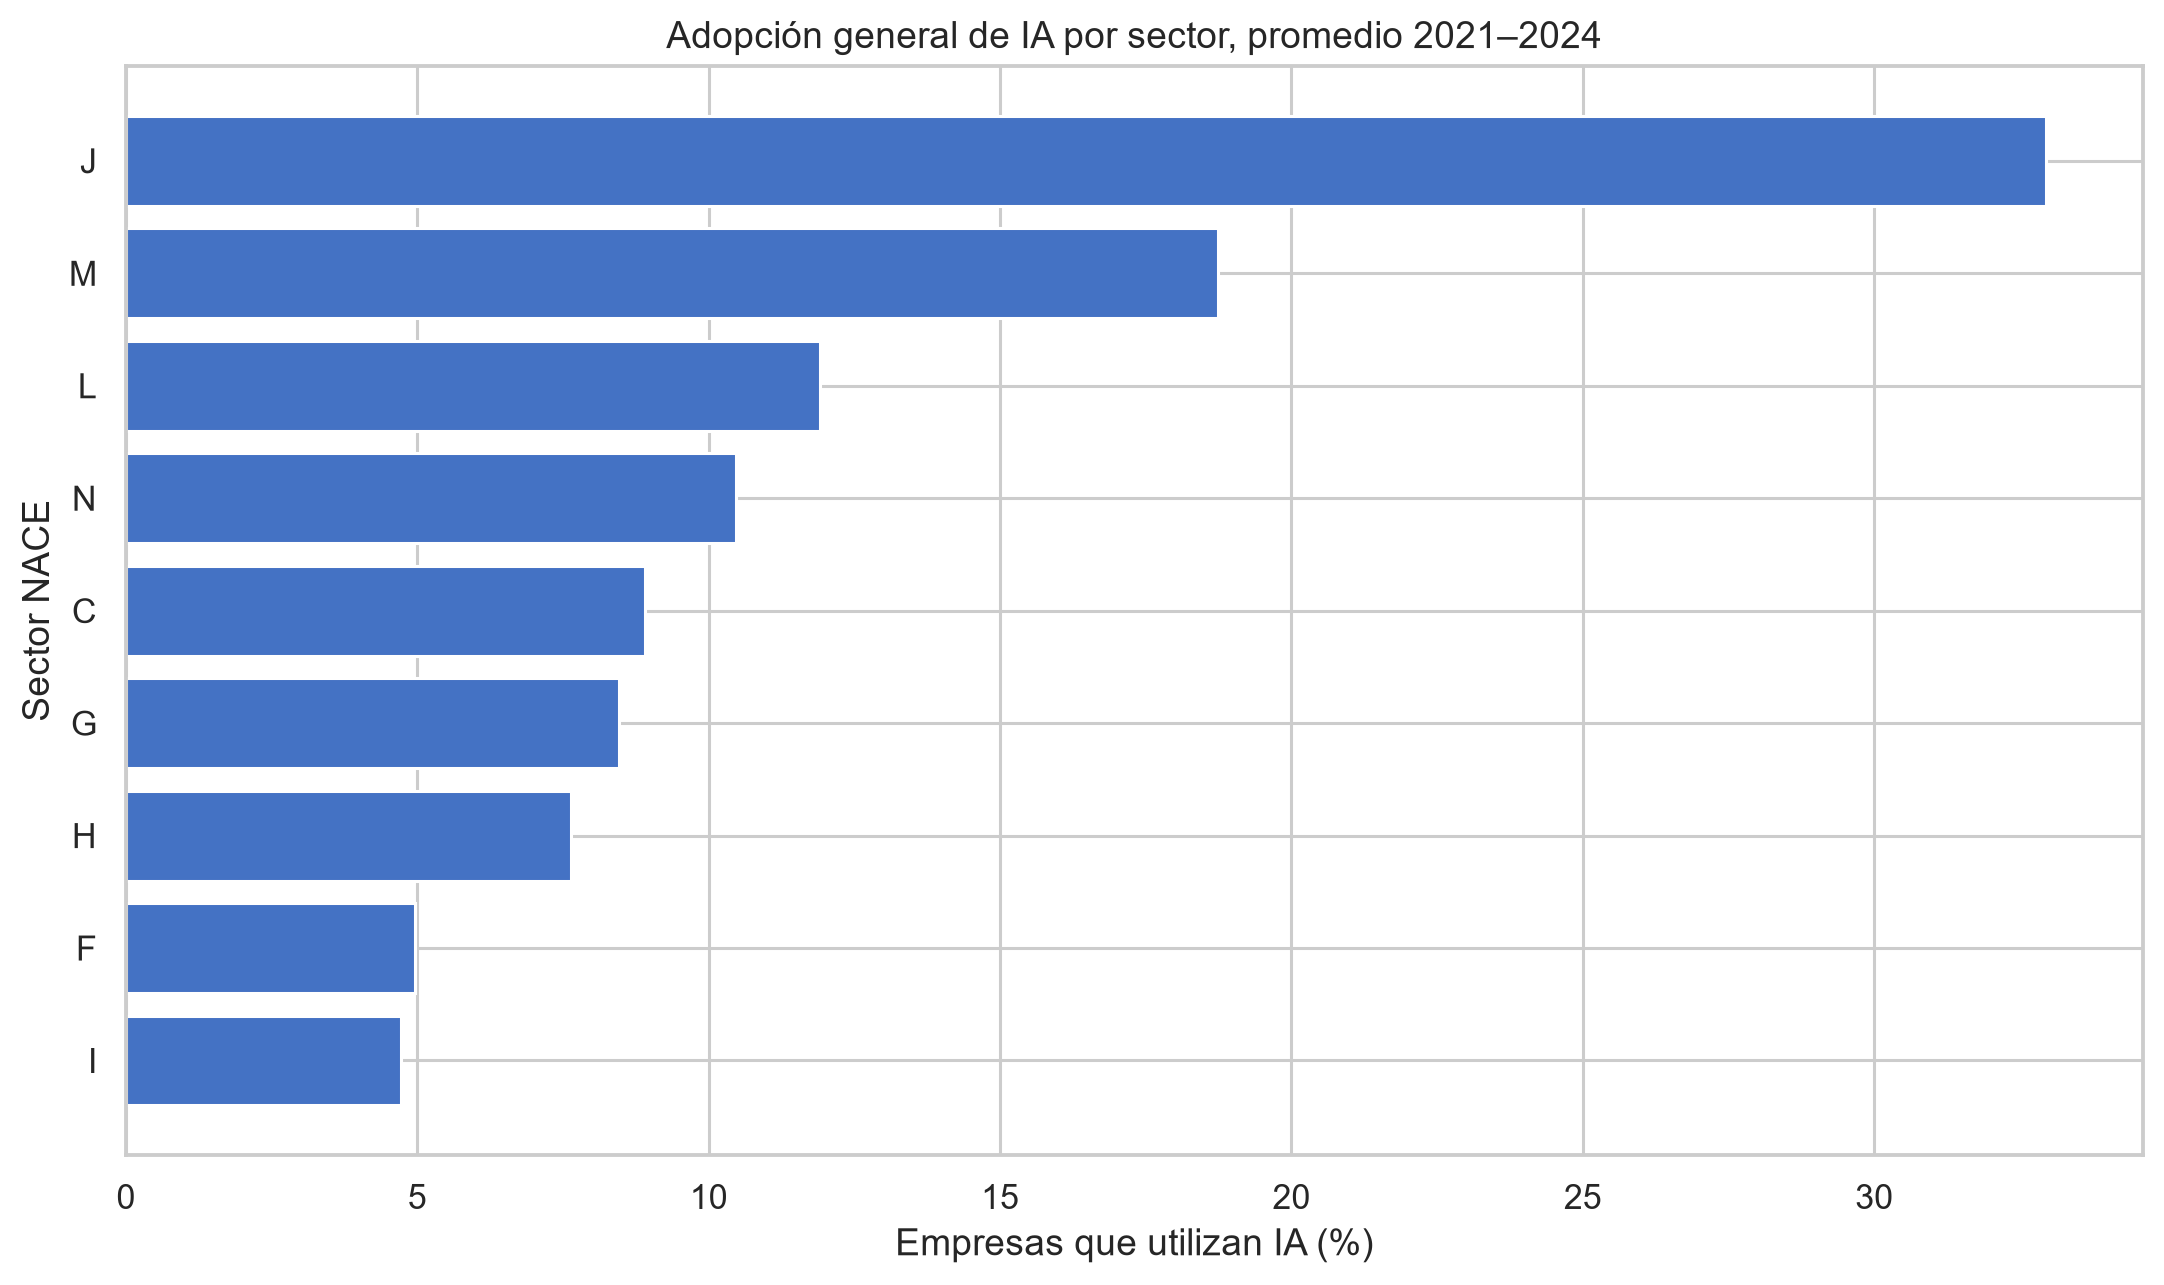
\includegraphics[width=0.9\linewidth]{../outputs/descriptivo_v0_1/figures/adopcion_ia_por_sector.png}
    \caption{Adopción general de IA por sector}
    \label{fig:adopcion-sector}
\end{figure}

\subsection{Correlaciones en niveles y cambios}

Las correlaciones en niveles entre indicadores de IA y log-productividad son positivas. Sin embargo, las correlaciones entre cambios de IA y cambios de log-productividad entre 2021 y 2024 son más débiles y, en varios casos, negativas. Esta diferencia sugiere que los sectores o países más productivos pueden adoptar más IA en promedio, sin que los aumentos recientes de adopción se traduzcan contemporáneamente en mayor crecimiento de productividad dentro de cada unidad observada.

\begin{table}[H]
\centering
\caption{Correlaciones entre IA y productividad}
\label{tab:correlaciones}
\small
\begin{tabular}{lrrrrr}
\toprule
\textbf{Indicador} & \textbf{Obs.} & \textbf{$r$ niveles} & \textbf{$p$} & \textbf{$r$ cambios} & \textbf{$p$} \\
\midrule
Adopción general & 627 & 0,564 & <0,001 & -0,217 & 0,002 \\
Dos o más tecnologías & 625 & 0,497 & <0,001 & -0,220 & 0,001 \\
Tres o más tecnologías & 615 & 0,463 & <0,001 & -0,209 & 0,003 \\
Procesos y decisiones & 624 & 0,533 & <0,001 & -0,059 & 0,399 \\
Producción & 597 & 0,504 & <0,001 & -0,135 & 0,061 \\
Logística & 590 & 0,418 & <0,001 & 0,027 & 0,715 \\
Marketing y ventas & 603 & 0,414 & <0,001 & -0,268 & <0,001 \\
Seguridad informática & 592 & 0,438 & <0,001 & -0,120 & 0,098 \\
\bottomrule
\end{tabular}
\begin{flushleft}
\footnotesize Nota: las correlaciones en niveles usan log-productividad. Las correlaciones de cambios corresponden a variaciones 2021--2024.
\end{flushleft}
\end{table}

\begin{figure}[H]
    \centering
    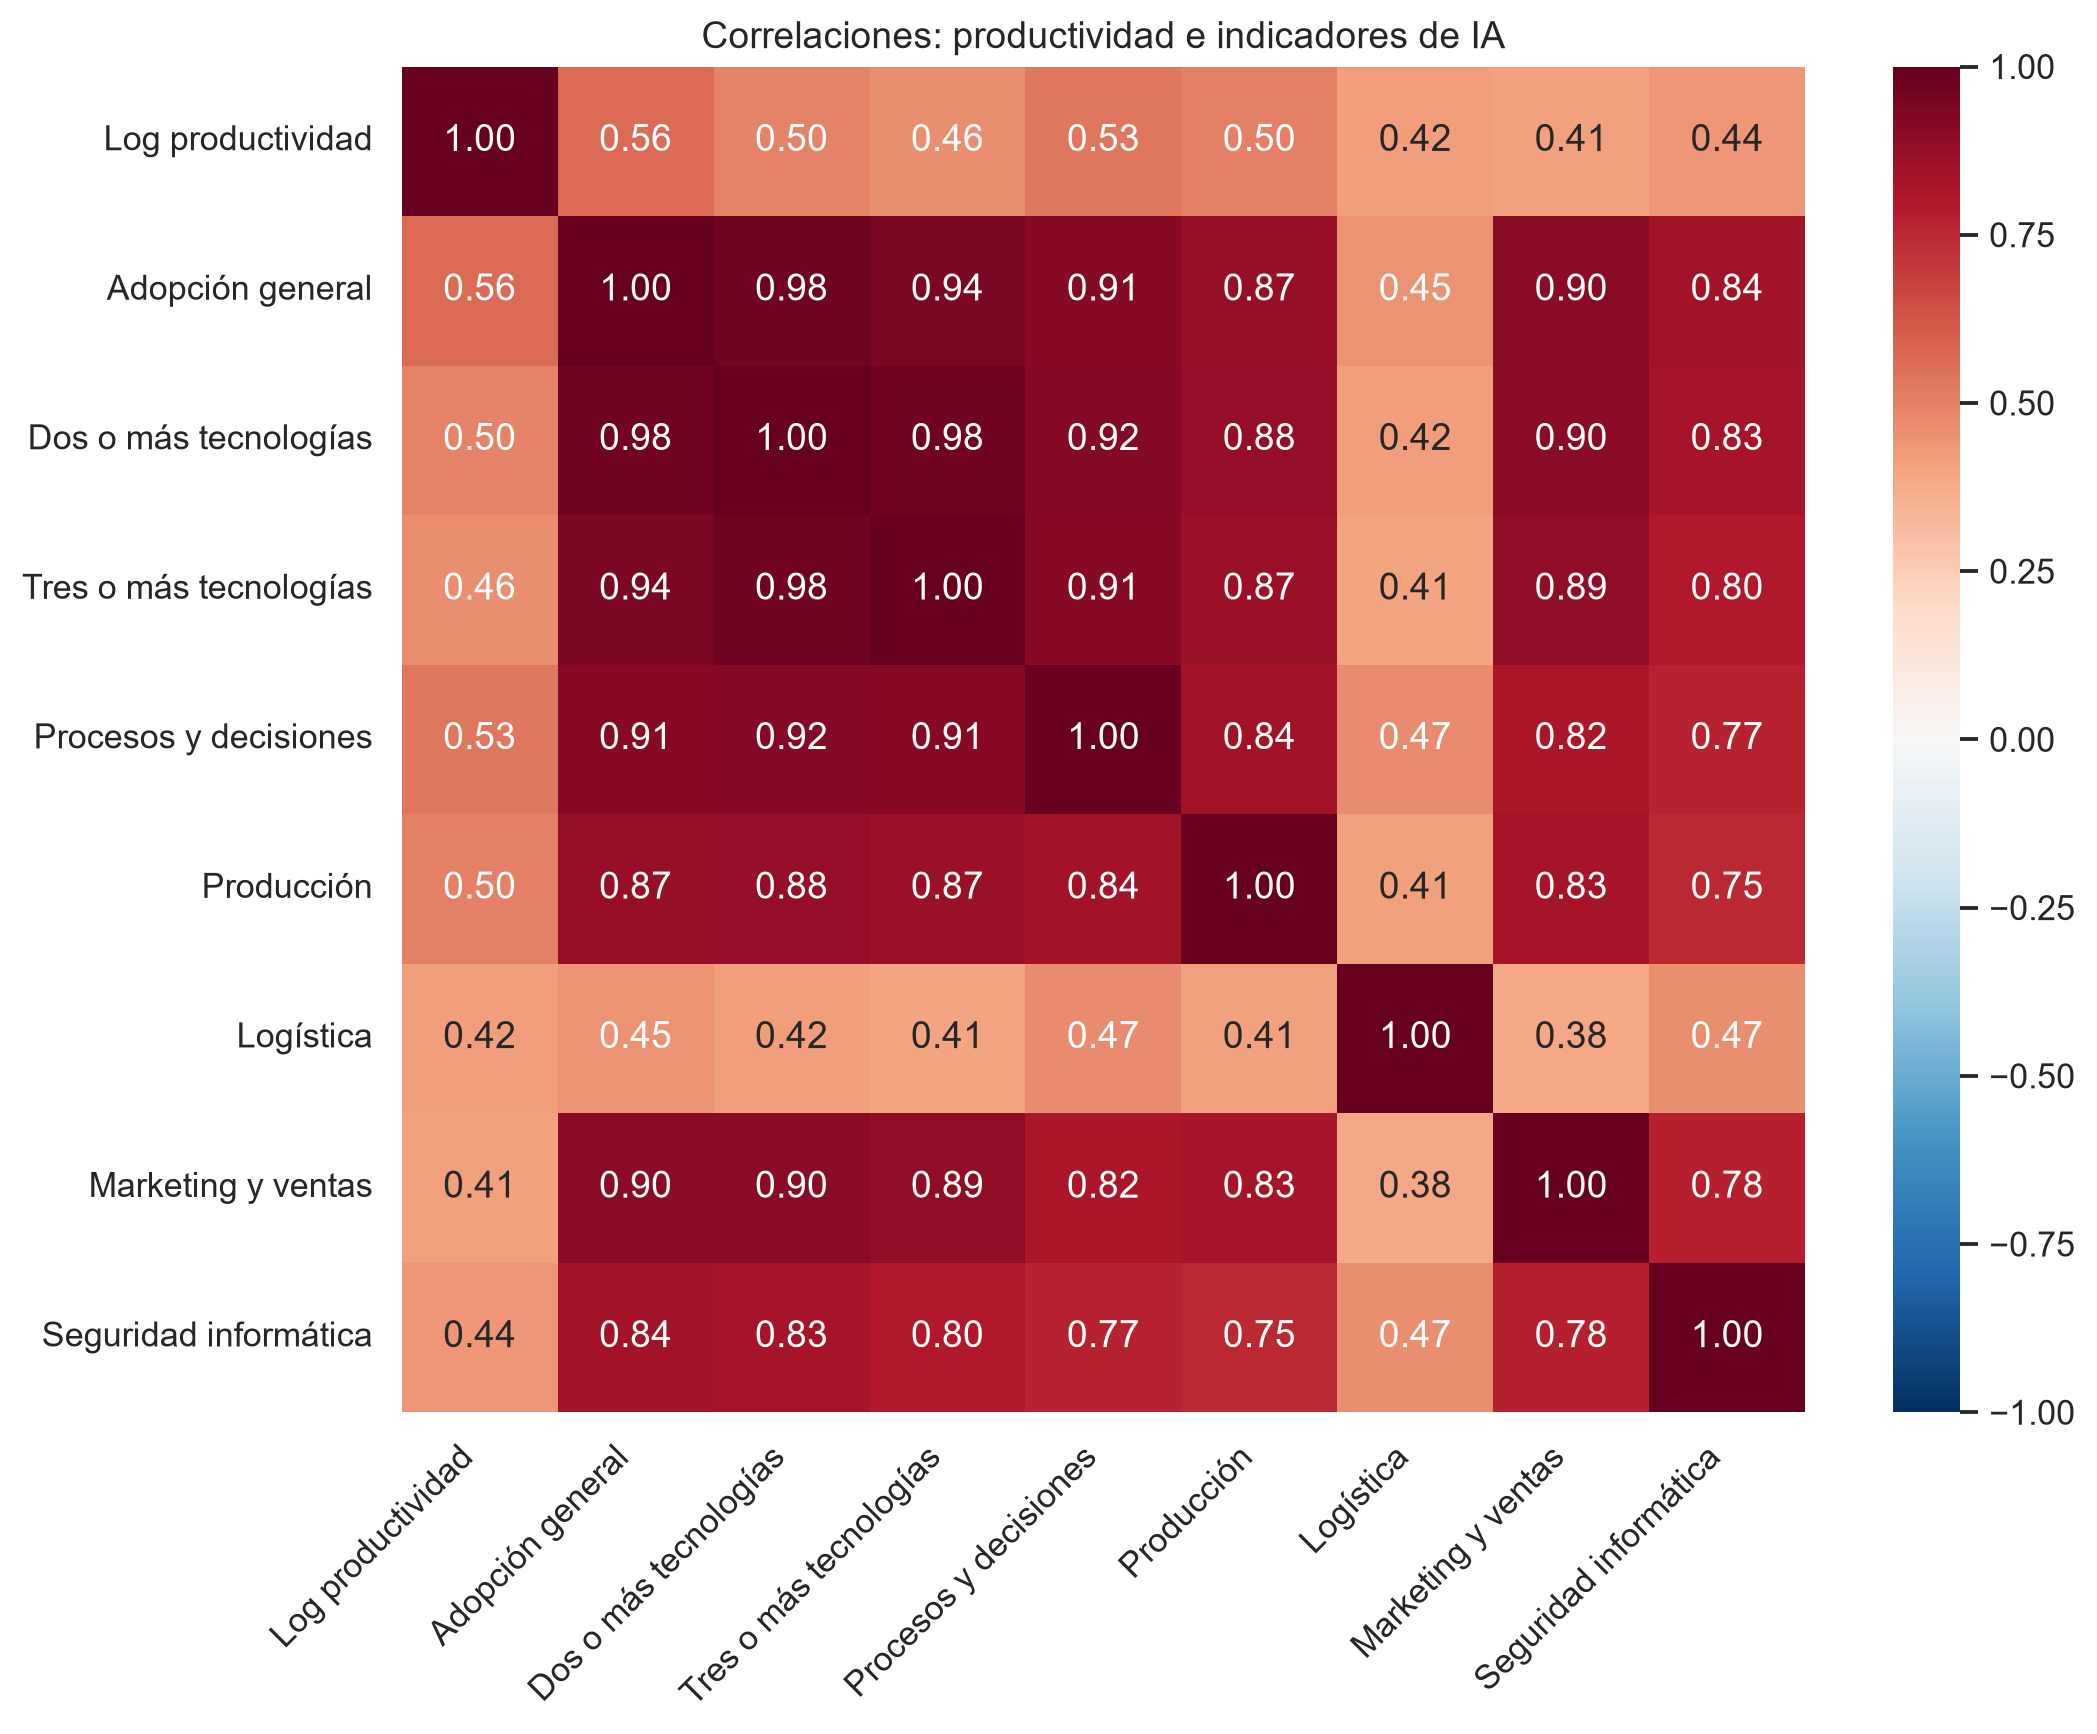
\includegraphics[width=0.85\linewidth]{../outputs/descriptivo_v0_1/figures/matriz_correlaciones.png}
    \caption{Matriz de correlaciones entre productividad e indicadores de IA}
    \label{fig:matriz-correlaciones}
\end{figure}

\subsection{Modelo de panel preliminar}

La especificación con efectos fijos de país--sector y país--año no arroja, en la estimación preliminar validada con \texttt{linearmodels}, coeficientes estadísticamente significativos para los indicadores de IA a niveles convencionales. La Tabla~\ref{tab:modelo-m3} reporta el modelo preferido. Para adopción general, el coeficiente estimado por un punto porcentual es aproximadamente -0,0011, con $n=627$ observaciones y 209 clusters país--sector. Interpretado para un aumento de 10 puntos porcentuales, el efecto estimado equivale aproximadamente a -1,1\%, aunque no es estadísticamente distinguible de cero.

\begin{table}[H]
\centering
\caption{Modelo M3: efectos fijos país--sector y país--año}
\label{tab:modelo-m3}
\small
\begin{tabular}{lrrrrr}
\toprule
\textbf{Indicador} & \textbf{$\beta$ 1 pp} & \textbf{EE} & \textbf{$p$} & \textbf{Efecto 10 pp} & \textbf{Obs.} \\
\midrule
Adopción general & -0,0011 & 0,0009 & 0,250 & -1,1 & 627 \\
Dos o más tecnologías & -0,0015 & 0,0010 & 0,120 & -1,5 & 625 \\
Tres o más tecnologías & -0,0019 & 0,0014 & 0,172 & -1,9 & 615 \\
Procesos y decisiones & -0,0003 & 0,0017 & 0,860 & -0,3 & 624 \\
Producción & -0,0011 & 0,0018 & 0,529 & -1,1 & 597 \\
Logística & 0,0010 & 0,0082 & 0,901 & 1,0 & 590 \\
Marketing y ventas & -0,0038 & 0,0021 & 0,078 & -3,7 & 603 \\
Seguridad informática & -0,0012 & 0,0024 & 0,610 & -1,2 & 592 \\
\bottomrule
\end{tabular}
\begin{flushleft}
\footnotesize Nota: variable dependiente: logaritmo de productividad laboral aparente. Errores estándar agrupados por entidad país--sector. Efecto 10 pp calculado como $100\times(\exp(10\beta)-1)$.
\end{flushleft}
\end{table}

Este resultado no debe interpretarse como evidencia de que la IA reduzca productividad ni como prueba de que la IA sea ineficaz. Indica que, bajo controles exigentes y con el horizonte temporal disponible, no se observa una asociación temporal positiva robusta. El patrón es compatible con diferencias estructurales, costos de ajuste, maduración lenta, inversiones complementarias, causalidad inversa, shocks sectoriales o limitaciones de medición.

\subsection{Robustez de la especificación principal}

Como prueba de sensibilidad inicial, se reestimó el modelo M3 para adopción general bajo cuatro decisiones alternativas: muestra balanceada sin ponderar, muestra central completa sin exigir balance, muestra balanceada ponderada por personas ocupadas y muestra balanceada excluyendo extremos p1--p99 de productividad. La Tabla~\ref{tab:robustez-adopcion} resume los resultados.

\begin{table}[H]
\centering
\caption{Robustez del modelo M3 para adopción general de IA}
\label{tab:robustez-adopcion}
\small
\begin{tabularx}{\textwidth}{Xrrrr}
\toprule
\textbf{Escenario} & \textbf{$\beta$ 1 pp} & \textbf{EE} & \textbf{$p$} & \textbf{Efecto 10 pp} \\
\midrule
Muestra balanceada, sin ponderar & -0,0011 & 0,0009 & 0,250 & -1,1 \\
Muestra central completa, sin ponderar & -0,0013 & 0,0009 & 0,154 & -1,3 \\
Muestra balanceada, ponderada por empleo & -0,0016 & 0,0008 & 0,038 & -1,6 \\
Muestra balanceada, sin extremos p1--p99 & -0,0007 & 0,0009 & 0,391 & -0,7 \\
\bottomrule
\end{tabularx}
\begin{flushleft}
\footnotesize Nota: variable dependiente: logaritmo de productividad laboral aparente. Todos los modelos incluyen efectos fijos país--sector y país--año. Errores estándar agrupados por entidad país--sector. Efecto 10 pp calculado como $100\times(\exp(10\beta)-1)$.
\end{flushleft}
\end{table}

El signo del coeficiente de adopción general se mantiene negativo en los cuatro escenarios, aunque sólo resulta estadísticamente significativo al 5\% en la estimación ponderada por empleo. Esta evidencia debe interpretarse con cautela: no demuestra un efecto negativo de la IA, pero sí indica que la ausencia de una asociación temporal positiva no depende exclusivamente de exigir una muestra balanceada ni de unos pocos valores extremos de productividad. La diferencia entre las asociaciones positivas en niveles y los modelos con controles exigentes sigue siendo el resultado interpretativo central.

\section{Discusión}

Los resultados preliminares refuerzan la necesidad de separar tres planos. Primero, la descripción de qué sectores y países adoptan más IA. Segundo, la asociación transversal entre adopción y productividad. Tercero, la variación dentro de cada unidad país--sector una vez controladas características permanentes y shocks país--año. Confundir estos planos puede llevar a conclusiones excesivas.

La correlación positiva en niveles es consistente con la idea de que las unidades más productivas también disponen de mayores capacidades para adoptar IA. La ausencia de una asociación positiva clara en variaciones internas no invalida el interés económico del fenómeno; más bien sugiere que la adopción declarada puede no ser suficiente para generar aumentos inmediatos de productividad observables en datos agregados. La realización productiva puede depender de la profundidad de integración, las tareas afectadas, la reorganización de procesos y otros activos complementarios no observados directamente en la base.

\section{Conclusiones preliminares}

Este trabajo propone analizar la relación entre usos empresariales de IA y productividad laboral aparente en sectores de la Unión Europea mediante una base país--sector--año construida con datos oficiales de Eurostat. El aporte esperado consiste en ordenar evidencia reproducible, distinguir adopción general de usos funcionales, comparar asociaciones en niveles y variaciones internas, y examinar heterogeneidad sectorial.

La evidencia preliminar muestra una asociación positiva en niveles entre IA y productividad, pero no una relación temporal robusta al controlar por efectos fijos de país--sector y país--año. Esta diferencia es central para la interpretación económica: adoptar IA no equivale necesariamente a obtener resultados productivos inmediatos, y los datos agregados no permiten diagnosticar la calidad de implementación ni el retorno de empresas individuales.

Las próximas etapas del trabajo consisten en auditar definitivamente la base, validar los modelos con herramientas econométricas estándar, ampliar el análisis de heterogeneidad sectorial, ejecutar robusteces predefinidas y completar la revisión bibliográfica. Las conclusiones finales deberán mantener una interpretación asociativa y prudente, evitando afirmar causalidad o realizar diagnósticos empresariales que los datos no permiten sostener.

\clearpage
\section{Bibliografía}
\renewcommand{\refname}{}
\bibliographystyle{apalike}
\bibliography{referencias}

\newpage
\section*{Anexo}
\addcontentsline{toc}{section}{Anexo}

Este anexo se reservará para documentación complementaria de datos, definiciones de variables, tablas adicionales, pruebas de robustez y detalles de reproducibilidad.

\end{document}
